\documentclass[tikz,border=10pt]{standalone}
\usepackage{amsmath,amssymb}
\usetikzlibrary{calc,arrows.meta}

\begin{document}
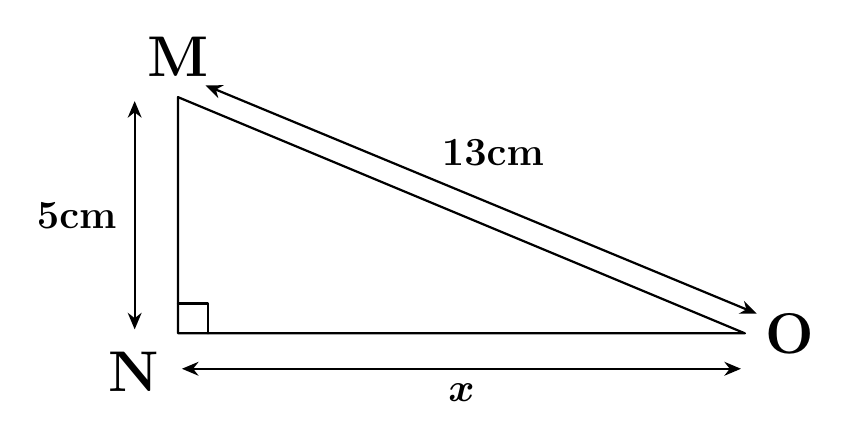
\begin{tikzpicture}[>=latex, line cap=round, line join=round]
  % Coordinates for exact 5:12:13 ratio (MN=3.0, NO=7.2, MO=7.8)
  \coordinate (N) at (0, 0);
  \coordinate (M) at (0, 3.0);
  \coordinate (O) at (7.2, 0);

  % Triangle boundary
  \draw[thick] (N) -- (M) -- (O) -- cycle;

  % Right-angle square at N
  \draw[thick] (0, 0.38) -- (0.38, 0.38) -- (0.38, 0);

  % Left vertical dimension line (5cm)
  \draw[{Stealth[length=6pt, width=5pt]}-{Stealth[length=6pt, width=5pt]}, thick] (-0.55, 0.05) -- (-0.55, 2.95);
  \node[left=3pt] at (-0.55, 1.5) {\Large $\mathbf{5cm}$};

  % Bottom horizontal dimension line (x)
  \draw[{Stealth[length=6pt, width=5pt]}-{Stealth[length=6pt, width=5pt]}, thick] (0.05, -0.45) -- (7.15, -0.45);
  \node[below=2pt] at (3.6, -0.45) {\Large $\boldsymbol{x}$};

  % Hypotenuse dimension line
  \coordinate (Mdim) at (0.35, 3.15);
  \coordinate (Odim) at (7.35, 0.25);
  \draw[{Stealth[length=6pt, width=5pt]}-{Stealth[length=6pt, width=5pt]}, thick] (Mdim) -- (Odim);

  % Horizontal label 13cm placed above the hypotenuse arrow
  \node at (4.0, 2.3) {\Large $\mathbf{13cm}$};

  % Vertex labels
  \node[above=4pt] at (M) {\huge $\mathbf{M}$};
  \node[below left=2pt] at (-0.05, -0.05) {\huge $\mathbf{N}$};
  \node[right=4pt] at (O) {\huge $\mathbf{O}$};

\end{tikzpicture}
\end{document}
